\documentclass{beamer}
\usefonttheme[onlymath]{serif}
\usetheme{Boadilla}
\usepackage{amsmath}
\usepackage{mathtools}
\title{Introduction to Neural Networks}
\subtitle{Day 2}
\author{Mohammad Khajah}
\institute[KISR]{Kuwait Institute for Scientific Research}
\date{}

\begin{document}

\begin{frame}
\titlepage
\end{frame}

\begin{frame}
\frametitle{Problem}

\begin{itemize}
\item Given the following data points, determine the relationship between $x$ and $y$, i.e., determine $y$ for arbitrary values of $x$.
\item Specifically, find a function $y(x)$ that maps $x$ to $y$.
\end{itemize}

\begin{figure}
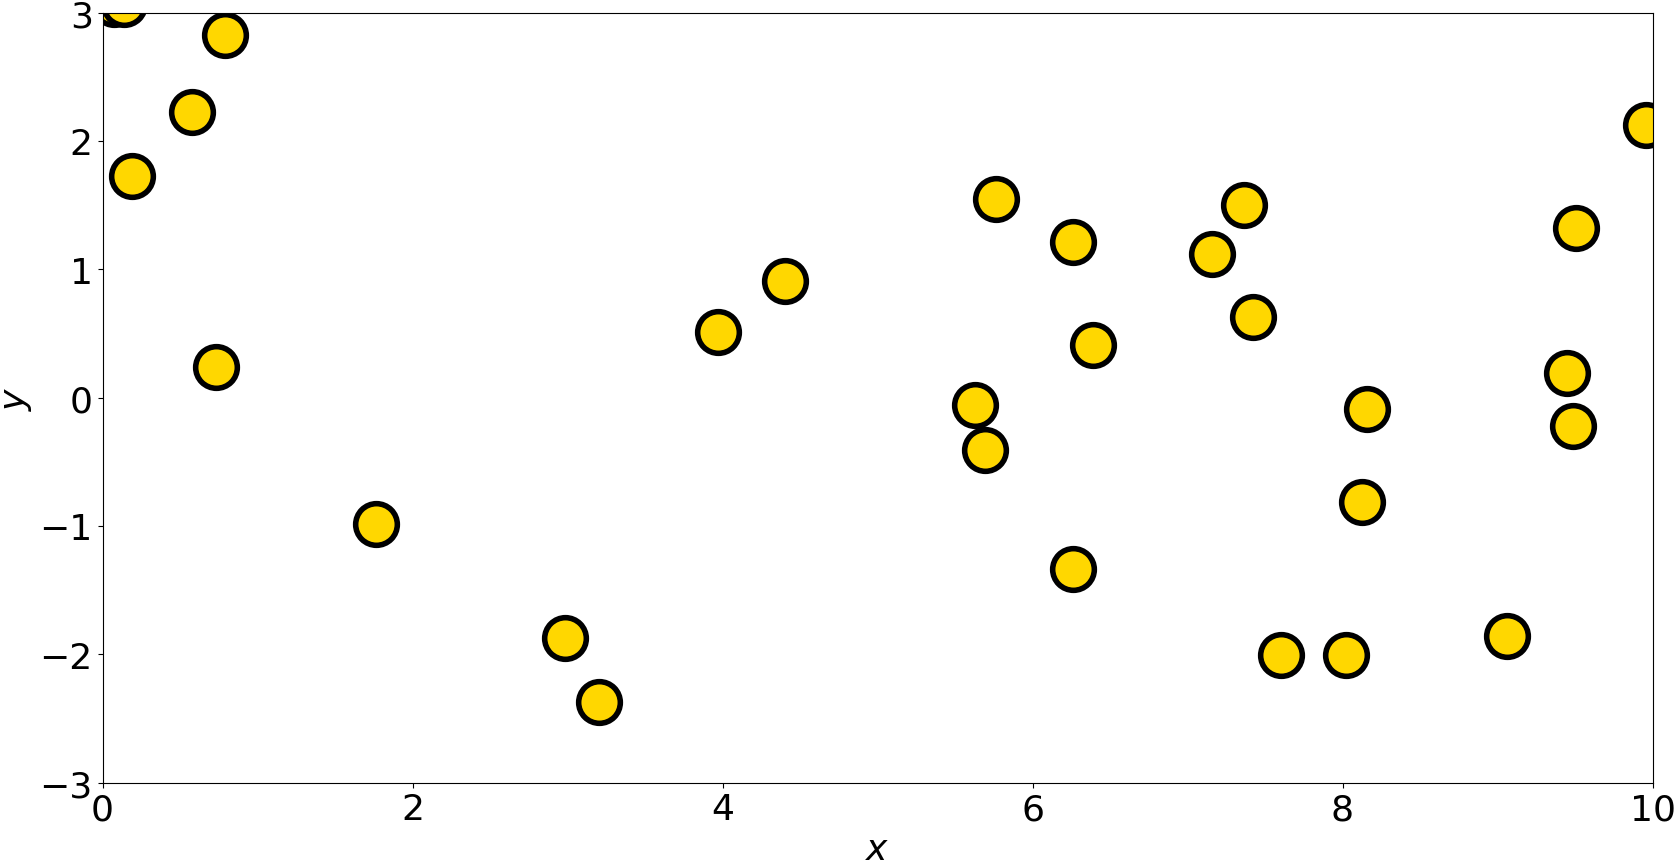
\includegraphics[width=0.85\textwidth]{../figures/fake_data.png}
\end{figure}

\end{frame}


\begin{frame}
\frametitle{First Attempt: Null Model}

\textbf{Simplest model}:  there is no relationship between $x$ and $y$

\begin{itemize}
\item $y$ remains constant as $x$ changes
\item But it appears that $y$ \textbf{does change} as $x$ changes!
\item Changes in $y$ are attributed to random noise $\epsilon$ (things that we can not account for)
\end{itemize}
\[
y(x) = c + \epsilon 
\]

``y has a constant level $c$ plus some random zero-mean noise"

\textbf{Prediction Equation}:  given $c$, the model's prediction is $\hat{y}(x) = c$

\begin{alertblock}{Task} 
How to find the free parameter $c$?
\end{alertblock}


\end{frame}

\begin{frame}
\frametitle{Loss Function}

\begin{columns}
\column{0.5\textwidth}

\begin{itemize}
\item There are infinitely many possible values of $c$
\item We'll use the data to find the best value of $c$ 
\item Need to score how good a particular value of $c$ is, given the data

\end{itemize}

\textbf{Idea}: average the lengths of all red lines. The greater the average, the worse the model. 

\begin{block}{Mean Absolute Error} 
\centering

$\mathcal{L}(\mathbf{y},\hat{\mathbf{y}})=\frac{1}{N}\sum_{i=1}^{N}\left|\hat{y}(x_{i})-y_{i}\right|$
\end{block}


\column{0.5\textwidth}

\begin{figure}
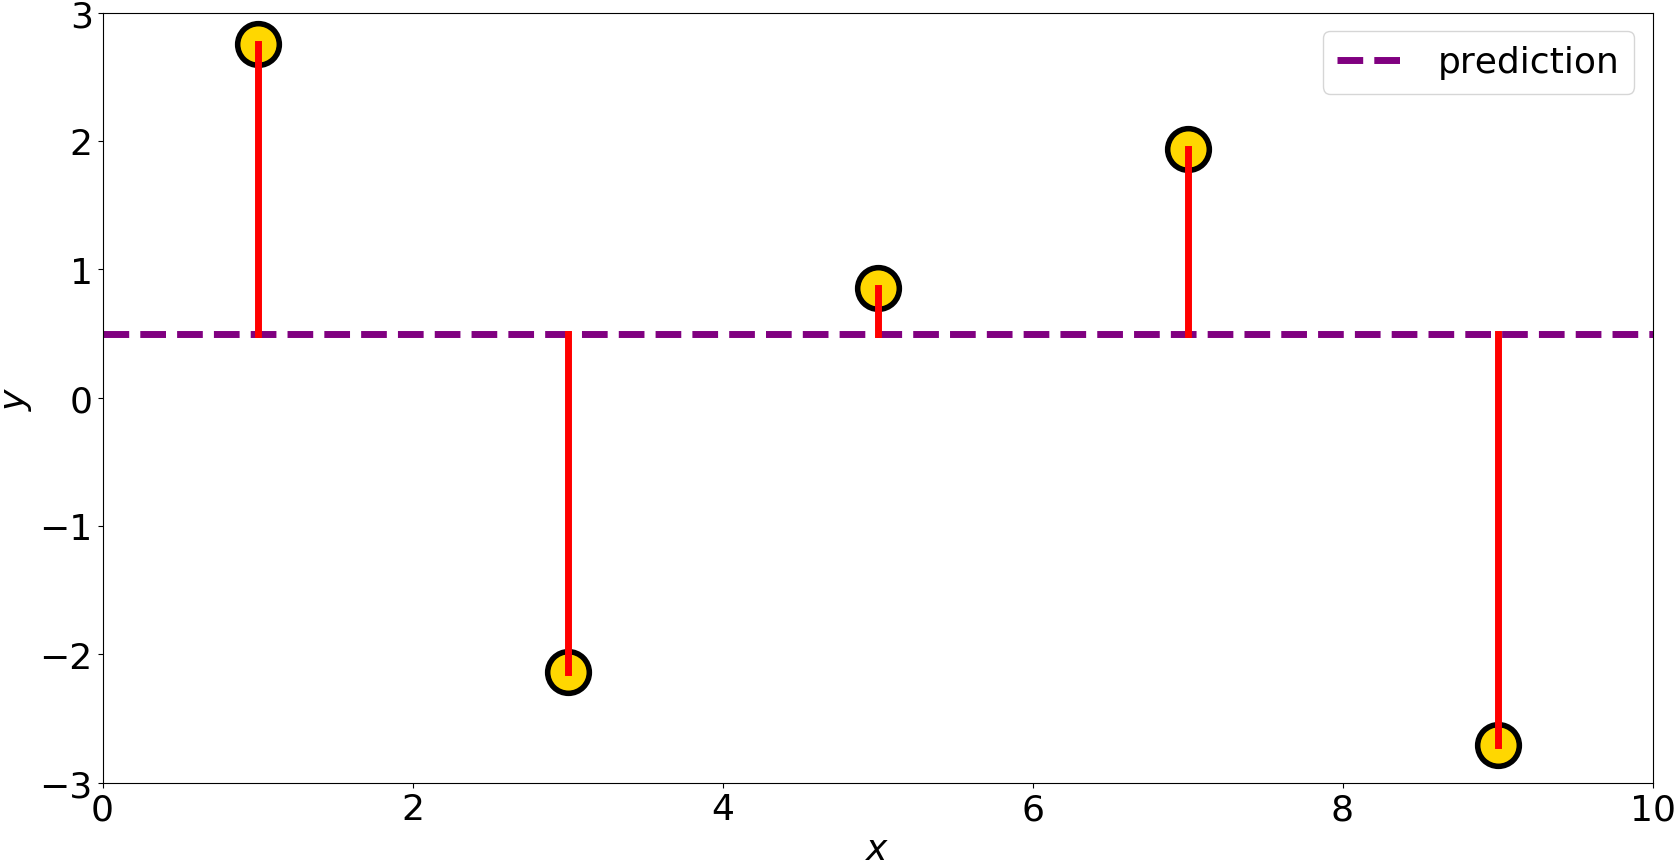
\includegraphics[width=\textwidth]{../figures/loss_demo.png}
\end{figure}

\end{columns}

\end{frame}


\begin{frame}
\frametitle{Minimizing the Loss Function}

\textbf{Objective}: find $c$ that minimizes MAE

\[
c^{*}=\underset{c}{\textrm{argmin}}\;\mathcal{L}(\mathbf{y},\hat{\mathbf{y}})
\]

We'll do this by brute force search:

\begin{enumerate}
\item pick a range of $c$ values to examine, e.g., $[-3, 3]$.
\item for each value of $c$ in the range:

\begin{enumerate}
\item compute model predictions $\hat{\mathbf{y}}$
\item compute $\mathcal{L}(\mathbf{y}, \hat{\mathbf{y}})$
\end{enumerate}

\item pick $c$ that has the smallest $\mathcal{L}(\mathbf{y}, \hat{\mathbf{y}})$

\end{enumerate}

\end{frame}

\begin{frame}
\frametitle{Implementation Time: Null Model}

\begin{itemize}
\item load the data from \texttt{fake\_data.npz} 
\item search for $c^*$ (best model fit)
\item plot the resulting best model fit along with the original data
\end{itemize}

\begin{exampleblock}{Result}
$c^* = 0.455$, smallest MAE: $1.350$
 \end{exampleblock}

\begin{figure}
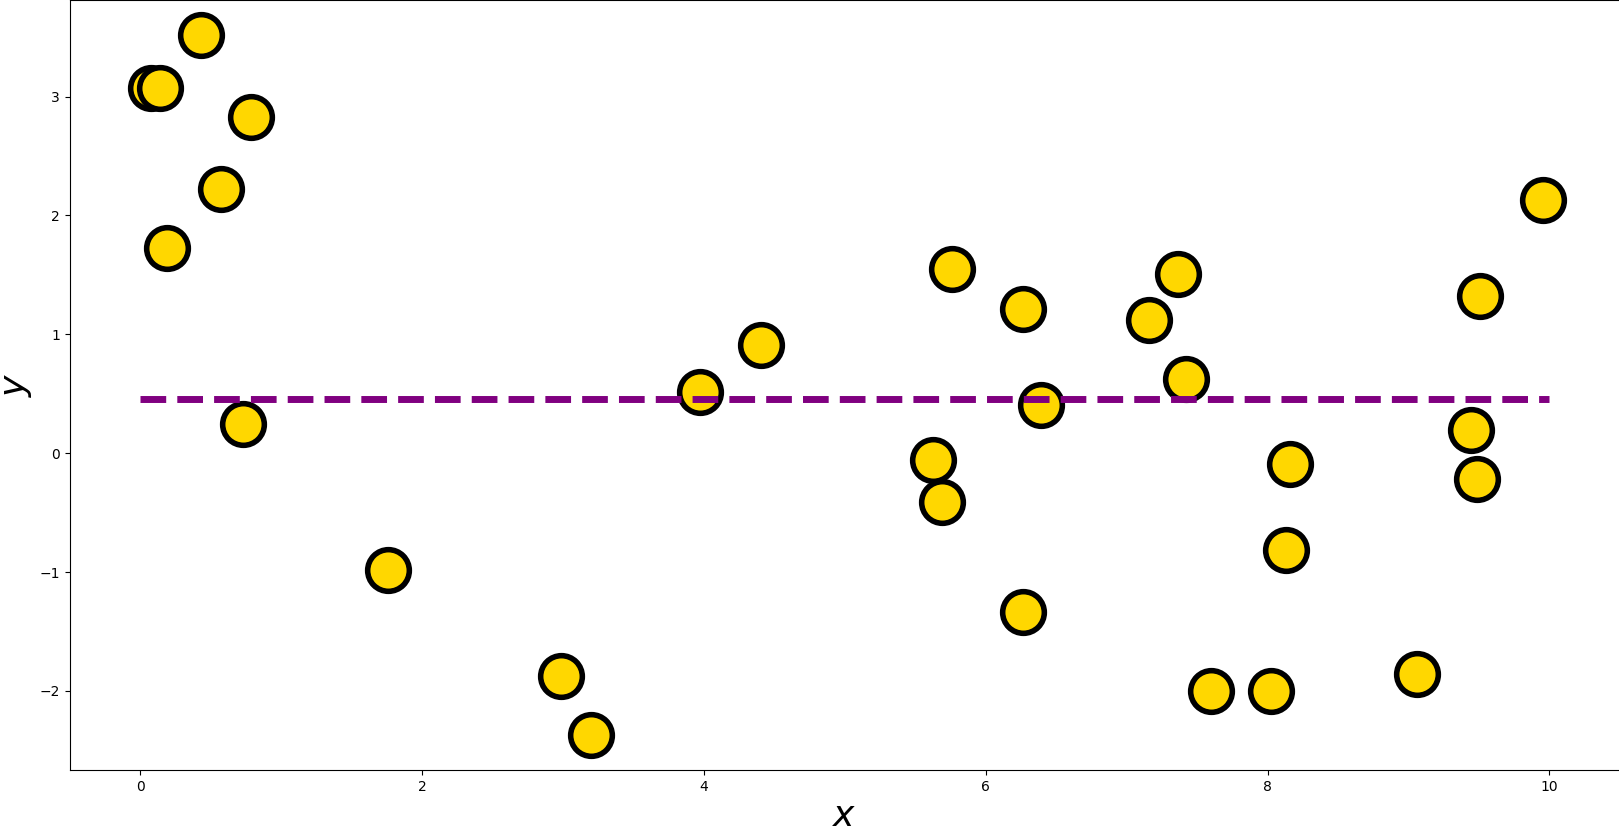
\includegraphics[width=0.55\textwidth]{../figures/best_null.png}
\end{figure}

\alert{Neat fact}: this is the \textbf{median} of the observations!

\end{frame}

\begin{frame}
\frametitle{Second Attempt: Linear Model}

\textbf{Can we do better?} surely, we can do better than a simple straight line!

Let's use a simple \emph{sloped} line instead.

\[
y(x)=\beta_{0}+\beta_{1}x+\epsilon
\]

\textbf{Number of Free Parameters}: 2

\textbf{Prediction Equation}: $\hat{y}(x) = \beta_0 + \beta_1 x$.

\textbf{Examples of lines for different combinations of $\beta_0$ and $\beta_1$}:

\begin{figure}
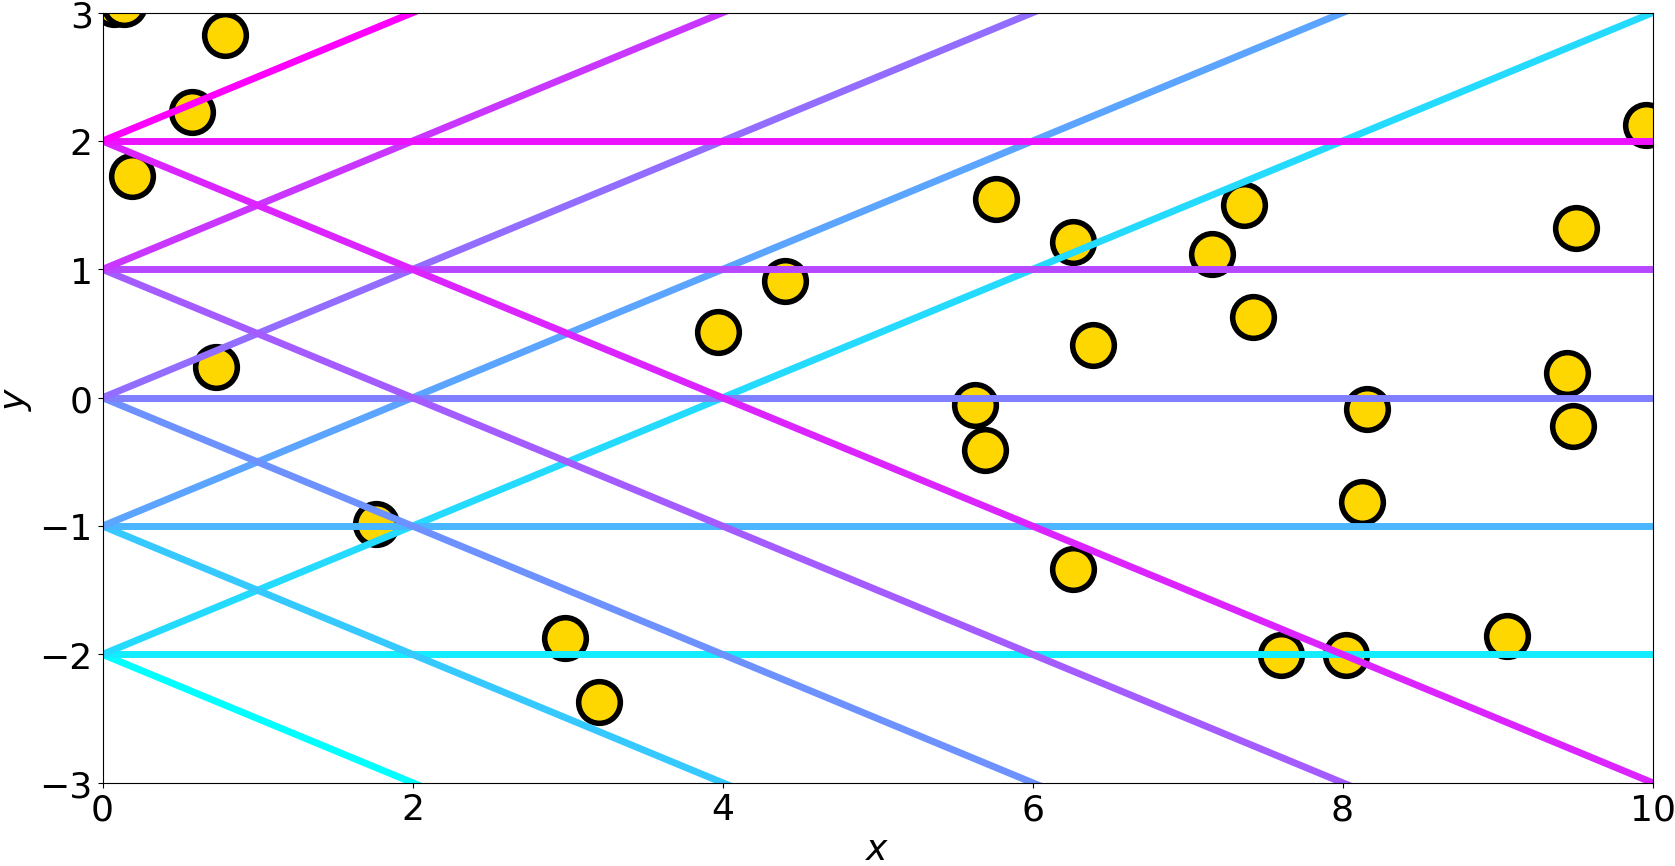
\includegraphics[width=0.55\textwidth]{../figures/line_priors.png}
\end{figure}


\end{frame}

\begin{frame}
\frametitle{Minimizing MAE for the Linear Model}

\begin{columns}
\column{0.5\textwidth}

\textbf{Objective}: find $\beta_0$ and $\beta_1$ that minimize MAE

\[
\boldsymbol{\beta}^{*}=\underset{\boldsymbol{\beta}}{\textrm{argmin}}\;\mathcal{L}(\mathbf{y},\hat{\mathbf{y}})
\]

We'll continue using brute force search by searching over possible combinations of $\beta_0$ and $\beta_1$.


\begin{block}{Number of Combinations} 
If we pick $100$ values for $\beta_0$ and $\beta_1$, the total number of combinations that need to be examined is $100 \times 100 = 10,000$.
\end{block}


\column{0.5\textwidth}

\begin{figure}
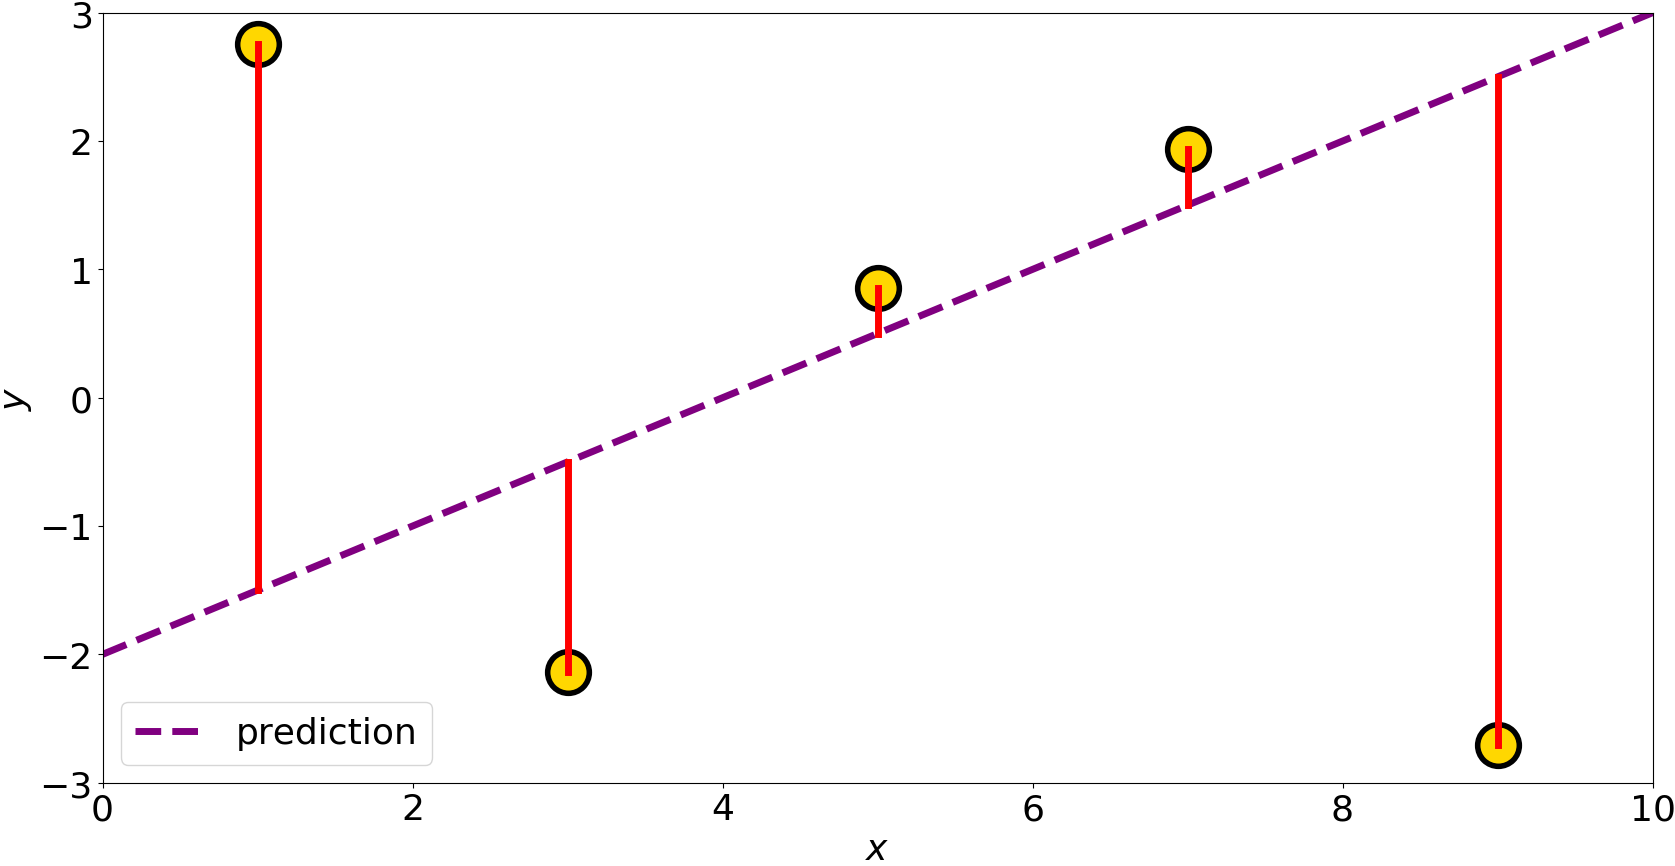
\includegraphics[width=\textwidth]{../figures/loss_demo_line.png}
\end{figure}

\end{columns}

\end{frame}


\begin{frame}
\frametitle{Implementation Time: Linear Model}

\begin{itemize}
\item load the data from \texttt{fake\_data.npz} 
\item search for $\boldsymbol{\beta}$ (best model fit)
\item plot the resulting best model fit along with the original data
\end{itemize}

\begin{exampleblock}{Result}
$\beta_0 = 1.788$, $\beta_1 =  -0.212$, smallest MAE: $1.206$
 \end{exampleblock}


\begin{figure}
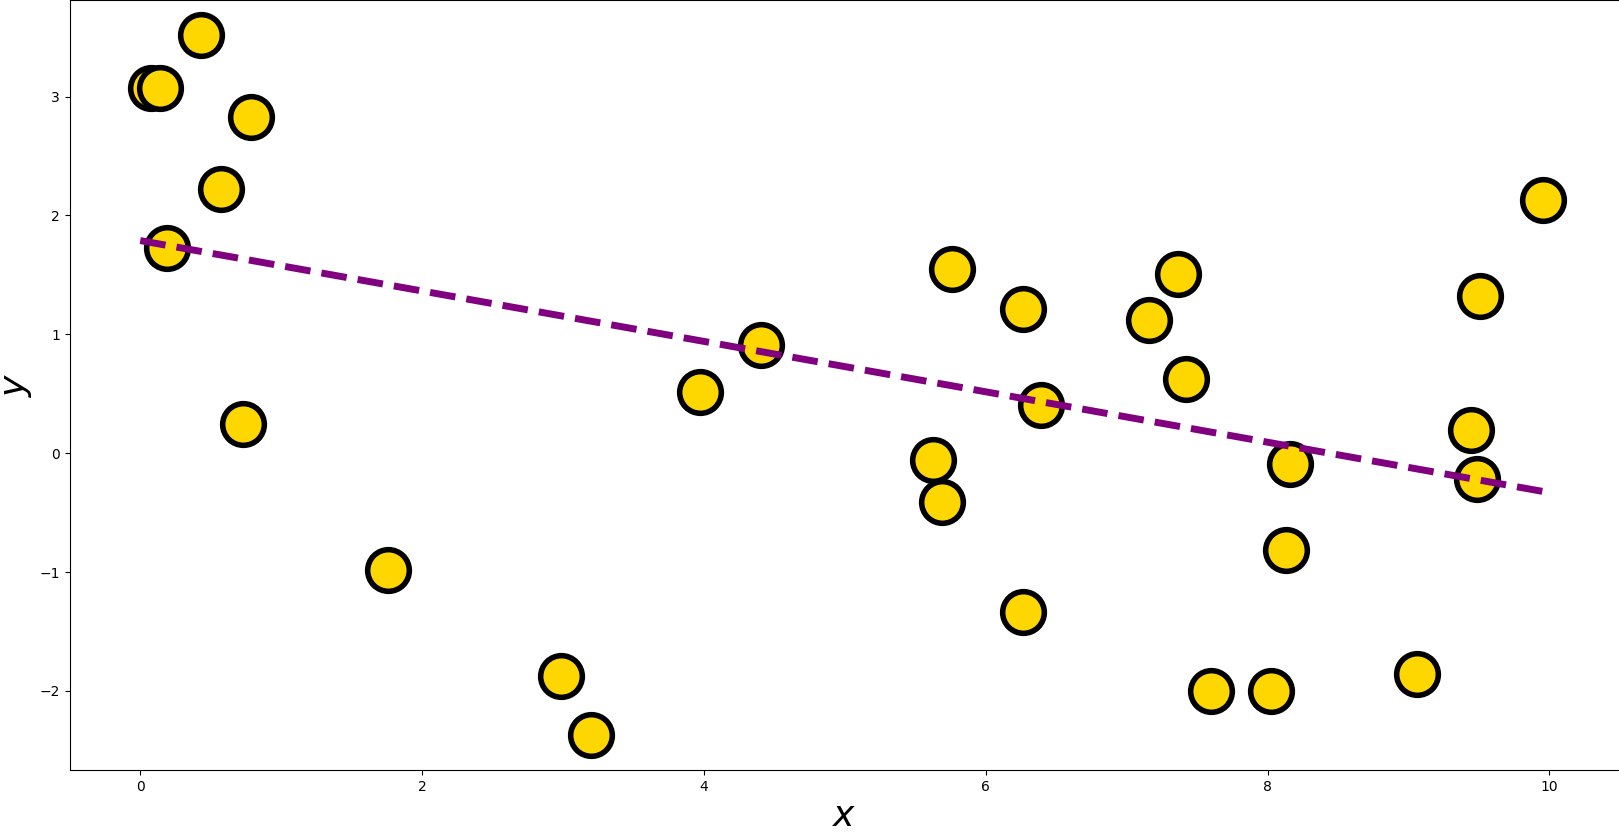
\includegraphics[width=0.55\textwidth]{../figures/best_linear.png}
\end{figure}

An \textbf{11\%} improvement over the null model.


\end{frame}

\begin{frame}
\frametitle{Problems with Brute Force Search}

\textbf{Combinatorial explosion}: as the number of free parameters increases, the number of combinations that have to be examined increases exponentially.

e.g., if there are $P$ free parameters, each with K values, the number of combinations is $K^P$.


\textbf{Choosing number of values}:
\begin{itemize}
\item \textbf{Too large}: slow search
\item \textbf{Too small}: might miss important minimums
\end{itemize}


\textbf{Why not just use calculus?} we are minimizing a function, so why not just take the derivative of the loss function, set it to zero, and find the minimum? 
\alert{Very difficult to do with more complicated models that we'll encounter later}

\begin{block}{Solution} 
We'll be seeking numerical solutions that minimize the loss function.
\end{block}

\end{frame}

\begin{frame}
\frametitle{Implementation: Visualize Loss of Null Model}

\begin{columns}

\column{0.5\textwidth}

Imagine dropping a ball at some random value of $c$, where would the ball go?
\begin{itemize}
\item if curve is flat, the ball stays
\item if curve is pointing up, the ball rolls backwards
\item if curve is pointing down, the ball rolls forwards
\end{itemize}

\textbf{Idea}: simulate the behavior of the ball. The ball stops moving when it is at a minimum.

\begin{alertblock}{Task}
How to compute steepness at any given point?
 \end{alertblock}

\column{0.5\textwidth}

\begin{figure}
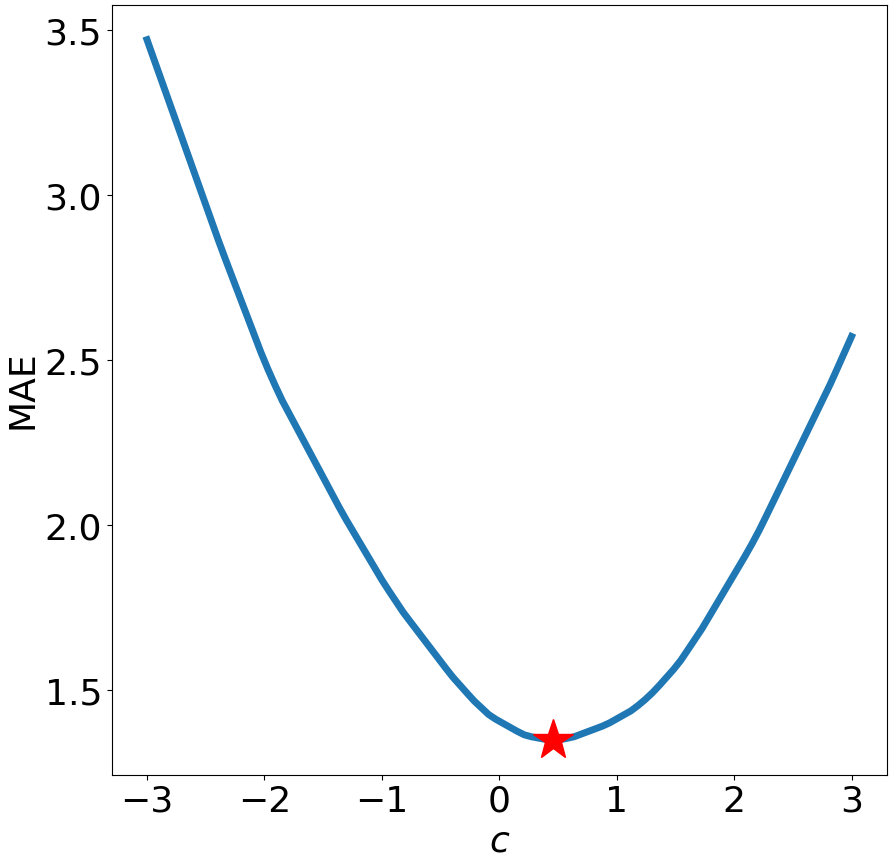
\includegraphics[width=\textwidth]{../figures/null_loss.png}
\end{figure}

\end{columns}

\end{frame}

\begin{frame}
\frametitle{Computing the Steepness of MAE for the Null Model}

\begin{itemize}
\item The steepness at a value $c$ corresponds to the slope at that point. 
\item The slope is just the first derivative of the loss function
\end{itemize}

\[
\frac{d}{dc}\mathcal{L}(\mathbf{y},\hat{\mathbf{y}})=\frac{1}{N}\sum_{i=1}^{N}\frac{d}{dc}\left|c-y_{i}\right|
\]

\[
\frac{d}{dc}\left|c-y_{i}\right|=\begin{cases}
1 & c-y_{i}>0\\
-1 & c-y_{i}<0
\end{cases}
\]

For a particular data point $y_i$:
\begin{itemize}
\item slope is positive if the model over predicts
\item slope is negative if the model under predicts
\end{itemize}

We call the derivative of the loss function the \textbf{The Gradient}
\end{frame}

\begin{frame}
\frametitle{Implementation: Visualize the Gradient of the Loss of the Null Model}


\begin{columns}

\column{0.5\textwidth}

Let's plot the gradient of the loss function as a function of $c$.

\begin{exampleblock}{Result}
\begin{itemize}
\item Gradient goes towards zeros as $c$ approaches optimal value
\item Gradient is largest (steepest) when $c$ is far from optimal
\end{itemize}
 \end{exampleblock}
 
\textbf{Idea}: simulate the motion of the ball by following the gradient.

\begin{itemize}
\item Gradient positive $\rightarrow$ decrease $c$
\item Gradient negative  $\rightarrow$  increase $c$
\end{itemize}

\column{0.5\textwidth}

\begin{figure}
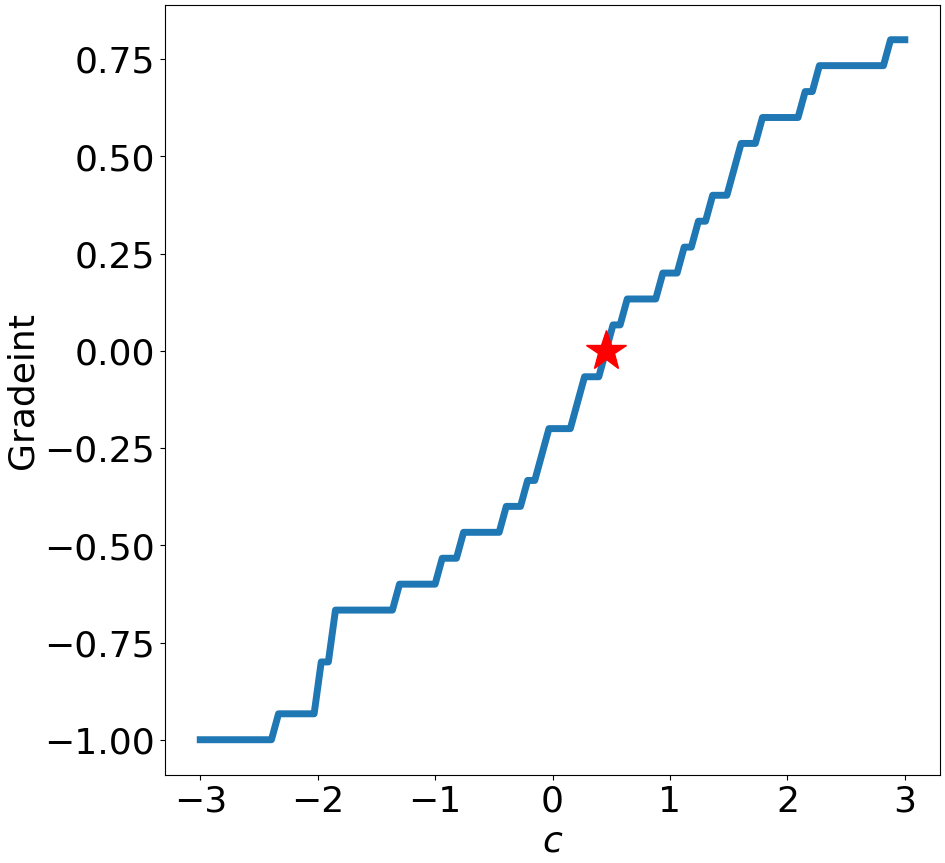
\includegraphics[width=\textwidth]{../figures/null_gradient.png}
\end{figure}

\end{columns}

\end{frame}

\begin{frame}
\frametitle{Gradient Descent}

\textbf{Gradient descent}:  an algorithm that numerically finds \alert{a local minimum} of a function by using the first derivative of the function.

\hfill

\begin{enumerate}
\item Initialize parameters $c$
\item Repeat until convergence

\begin{enumerate}
\item Compute model predictions $\hat{\boldsymbol{y}}$
\item Compute the gradient $\frac{d}{dc}\mathcal{L}(\mathbf{y},\hat{\mathbf{y}})$
\item Update $c$:

\[
c \coloneqq c-\eta\frac{d}{dc}\mathcal{L}(\mathbf{y},\hat{\mathbf{y}})
\]

\end{enumerate}

\end{enumerate}

\begin{block}

\begin{itemize}
\item The negative sign means to move opposite direction of the gradient
\item $\eta$ is the \textbf{learning rate} which controls the size of the steps the algorithm makes
\end{itemize}

\end{block}

\end{frame}


\begin{frame}
\frametitle{Implementation: Gradient Descent for the Null Model}

\begin{itemize}
\item Implement and run gradient descent for the null model (15 Iterations)
\item Plot progress for different learning rates
\end{itemize}


\centering
Starting from $c = 2.5$

\begin{tabular}{|c|c|c|}
\hline 
$\eta$ & $c^{*}$ & MAE\tabularnewline
\hline 
\hline 
0.1 & 1.553 & 1.595\tabularnewline
\hline 
\textbf{1.0} & \textbf{0.500} & \textbf{1.350}\tabularnewline
\hline 
3.0 & -1.167 & 1.935\tabularnewline
\hline 
\end{tabular}

\begin{figure}
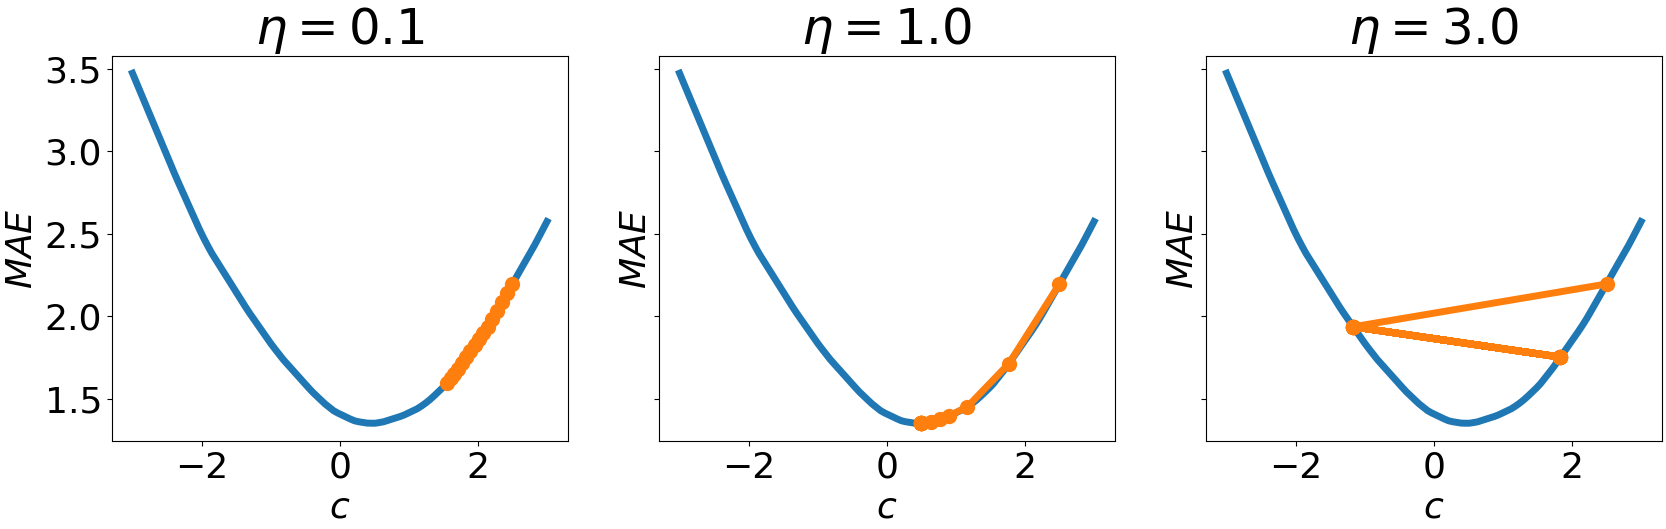
\includegraphics[width=\textwidth]{../figures/null_gd_steps.png}
\end{figure}

\end{frame}

\begin{frame}
\frametitle{Note on the Learning Rate}

\begin{block}

\begin{itemize}
\item There is no universal optimal learning rate, it depends on the model, data, and loss
\item There are schemes that adapt learning rate: start with large rate then reduce as learning progresses
\item For now, we'll use fixed learning rate
\end{itemize}

\end{block}

\begin{alertblock}{Question}
How to do gradient descent with the linear model?
\end{alertblock}

\end{frame}

\begin{frame}
\frametitle{Implementation: Visualize the Loss of the Linear Model}

Visualize linear model loss both in 3d and 2d.

\begin{figure}
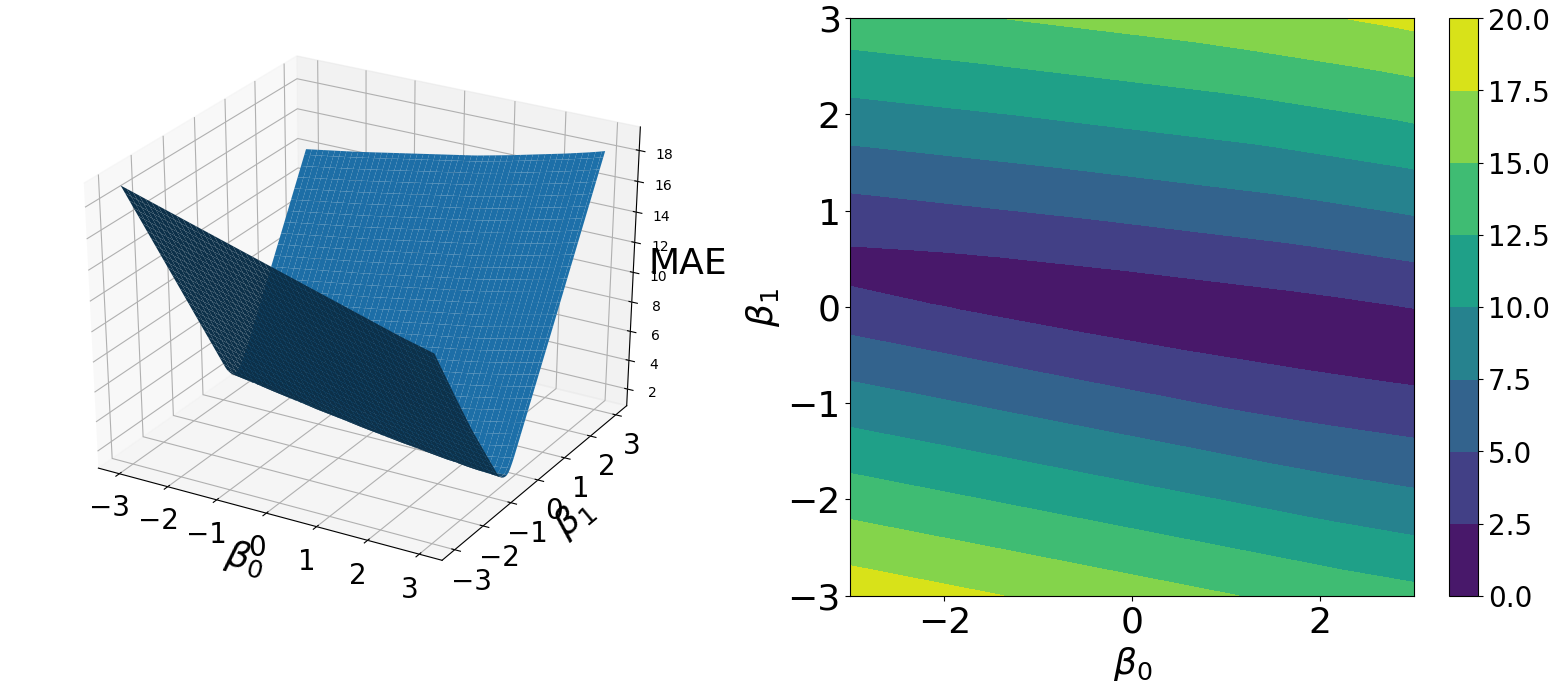
\includegraphics[width=\textwidth]{../figures/linear_loss.png}
\end{figure}


\end{frame}

\begin{frame}
\frametitle{Gradient Descent for the Linear Model}

For models with multiple parameters, take the \emph{partial} derivative of the loss with respect to each parameter. 

\[
\frac{\partial}{\partial\beta_{k}}\mathcal{L}(\mathbf{y},\hat{\mathbf{y}})=\frac{1}{N}\sum_{i=1}^{N}\frac{\partial}{\partial\beta_{k}}\left|\beta_{0}+\beta_{1}x_{i}-y_{i}\right|
\]

\[
\frac{\partial}{\partial\beta_{0}}\left|\beta_{0}+\beta_{1}x_{i}-y_{i}\right|=\begin{cases}
1 & \beta_{0}+\beta_{1}x_{i}-y_{i}>0\\
-1 & \beta_{0}+\beta_{1}x_{i}-y_{i}<0
\end{cases}
\]

\[
\frac{\partial}{\partial\beta_{1}}\left|\beta_{0}+\beta_{1}x_{i}-y_{i}\right|=\begin{cases}
x_{i} & \beta_{0}+\beta_{1}x_{i}-y_{i}>0\\
-x_{i} & \beta_{0}+\beta_{1}x_{i}-y_{i}<0
\end{cases}
\]

\[
\left[\begin{array}{c}
\beta_{0}\\
\beta_{1}
\end{array}\right]\coloneqq\left[\begin{array}{c}
\beta_{0}\\
\beta_{1}
\end{array}\right]-\eta\left[\begin{array}{c}
\frac{\partial}{\partial\beta_{0}}\mathcal{L}(\mathbf{y},\hat{\mathbf{y}})\\
\frac{\partial}{\partial\beta_{1}}\mathcal{L}(\mathbf{y},\hat{\mathbf{y}})
\end{array}\right]
\]

\end{frame}

\begin{frame}
\frametitle{Implementation: Gradient Descent with Linear Model}

\begin{itemize}
\item Run gradient descent for the linear model (500 iterations)
\item Plot progress on the contour plot for various learning rates
\end{itemize}

\centering
Starting from $\beta_0 = -2.0, \beta_1 = 2.5$

\begin{tabular}{|c|c|c|c|}
\hline 
$\eta$ & 0.01 & \textbf{0.05} & 2.0\tabularnewline
\hline 
\hline 
MAE & 1.627 & \textbf{1.231} & 2.357\tabularnewline
\hline 
\end{tabular}


\begin{figure}
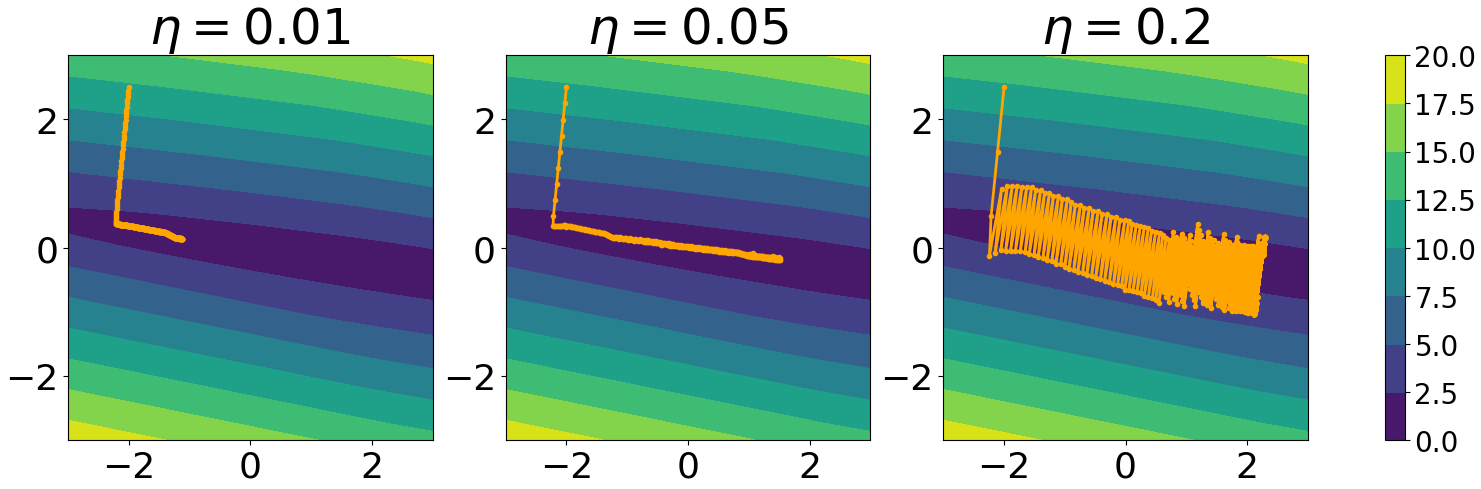
\includegraphics[width=\textwidth]{../figures/linear_gd_steps.png}
\end{figure}


\end{frame}

\begin{frame}
\frametitle{Third Attempt: Nonlinear Model}

An expert tells us that a better model should have the following form:
\begin{align*}
g(x) & =cos(\beta_{0}+\beta_{1}x)\\
\hat{y}(x) & =\gamma_{0}+\gamma_{1}g(x)
\end{align*}

\begin{enumerate}
\item The input $x$ is  transformed via $g(x)$
\item The output of $g(x)$ is then transformed via $\hat{y}(x)$
\end{enumerate}

\begin{figure}
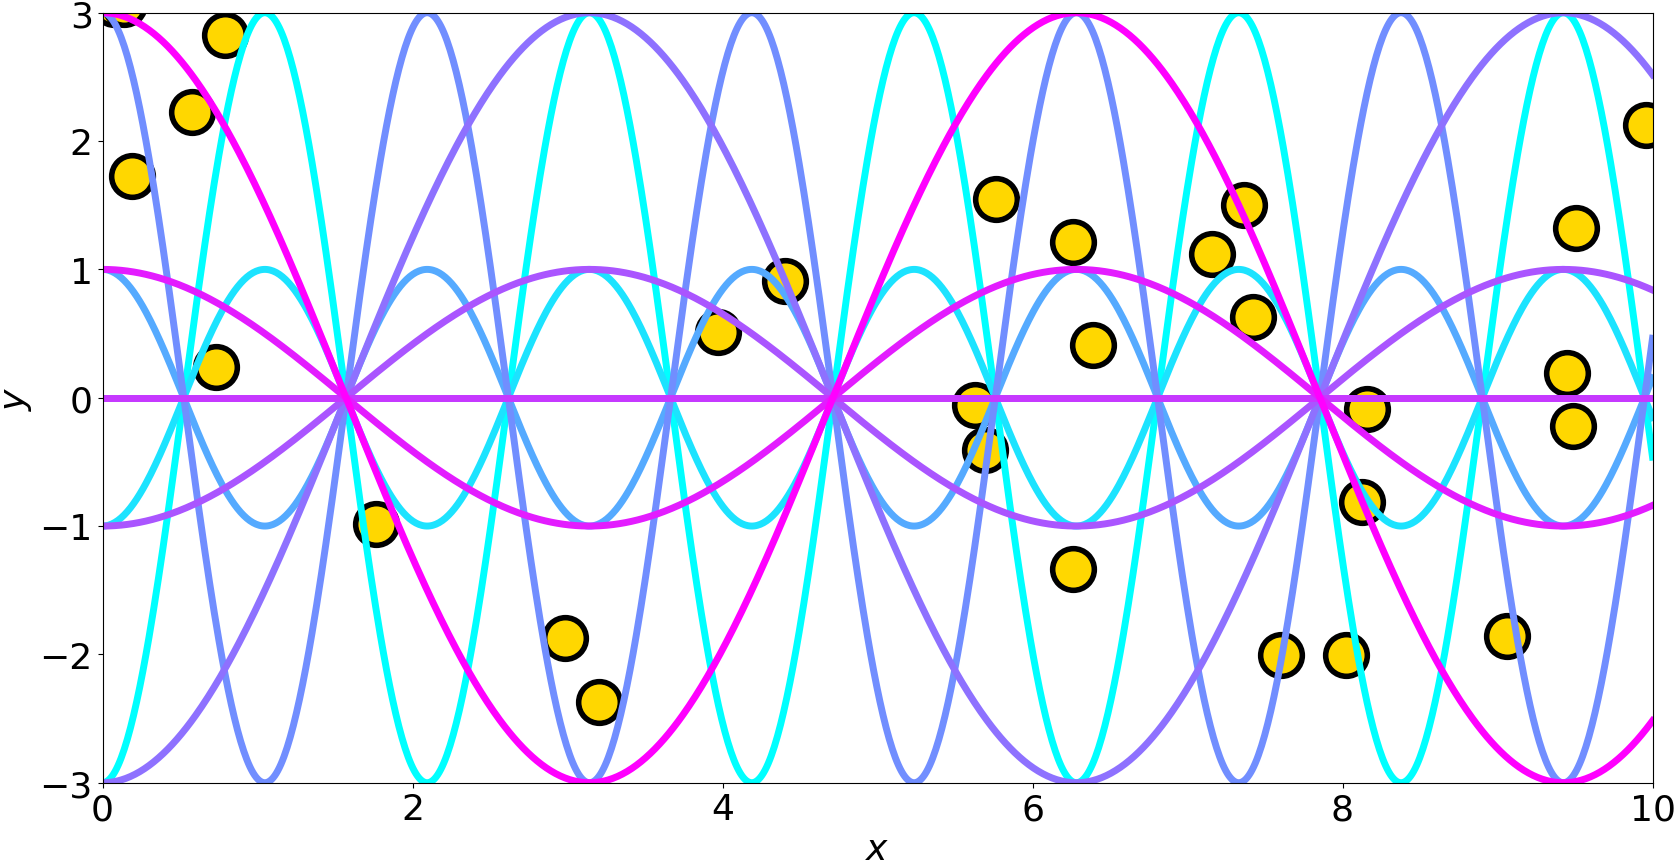
\includegraphics[width=0.65\textwidth]{../figures/nonlinear_priors.png}
\end{figure}

\end{frame}

\begin{frame}
\frametitle{Nonlinear Model Gradient Computations - I}

Let's revise the math notation a bit to make it easier to show gradient equations. MAE is:

\[
\mathcal{L}(\mathbf{y},\hat{\mathbf{y}})=\frac{1}{N}\sum_{i=1}^{N}\mathcal{L}(y_{i},\hat{y}_{i})
\]
\[
\mathcal{L}(y_{i},\hat{y}_{i})=\left|y_{i}-\hat{y}_{i}\right|
\]

\hfill 

and we are interested in $\frac{\partial}{\partial\theta_{k}}\mathcal{L}(y_{i},\hat{y}_{i})$ for each parameter $\theta_k$ in the model (we have 4 parameters in the nonlinear model from the previous slide).

\end{frame}

\begin{frame}
\frametitle{Nonlinear Model Gradient Computations - II}

First, let's do the easy gradients: those with respect to the parameters nearest to the output, $\gamma_0$ and $\gamma_1$.

\[
\frac{\partial}{\partial\gamma_{0}}\mathcal{L}(y_{i},\hat{y}_{i})=\begin{cases}
1 & \hat{y}(x_{i})-y_{i}>0\\
-1 & \hat{y}(x_{i})-y_{i}<0
\end{cases}
\]

\[
\frac{\partial}{\partial\gamma_{1}}\mathcal{L}(y_{i},\hat{y}_{i})=\begin{cases}
g(x) & \hat{y}(x_{i})-y_{i}>0\\
-g(x) & \hat{y}(x_{i})-y_{i}<0
\end{cases}
\]

Now, how to handle $\beta_0$ and $\beta_1$?

\begin{block}{Chain Rule}
If $z$ depends on $y$ and $y$ depends on $x$, then:
\[
\frac{dz}{dx}=\frac{dz}{dy}.\frac{dy}{dx}
\]
\end{block}

\end{frame}

\begin{frame}
\frametitle{Nonlinear Model Gradient Computations - III}

\[
\frac{\partial}{\partial\beta_{0}}\mathcal{L}(y_{i},\hat{y}_{i})=\frac{\partial\mathcal{L}}{\partial g}\frac{\partial g}{\partial\beta_{0}}=\begin{cases}
-\gamma_{1}sin(\beta_0 + \beta_1x) & \hat{y}_{i}-y_{i}>0\\
\gamma_{1}sin(\beta_0 + \beta_1x) & \hat{y}_{i}-y_{i}<0
\end{cases}
\]

\[
\frac{\partial}{\partial\beta_{1}}\mathcal{L}(y_{i},\hat{y}_{i})=\frac{\partial\mathcal{L}}{\partial g}\frac{\partial g}{\partial\beta_{1}}=\begin{cases}
-\gamma_{1}xsin(\beta_0 + \beta_1x) & \hat{y}_{i}-y_{i}>0\\
\gamma_{1}xsin(\beta_0 + \beta_1x) & \hat{y}_{i}-y_{i}<0
\end{cases}
\]

\end{frame}

\begin{frame}
\frametitle{Implementation: Nonlinear Model Gradient Descent}

\begin{itemize}
\item Implement and run gradient descent on the nonlinear model (10,000 iterations, $\eta = 0.01$)
\item Plot best fitting model
\end{itemize}

\begin{exampleblock}{Result}
\begin{itemize}
\item Sometimes the best MAE is 1.014
\item Sometimes it is 1.117 (shown here)
\end{itemize}
 \end{exampleblock}
 
 \begin{columns}
 
 \column{0.5\textwidth}
 \begin{figure}
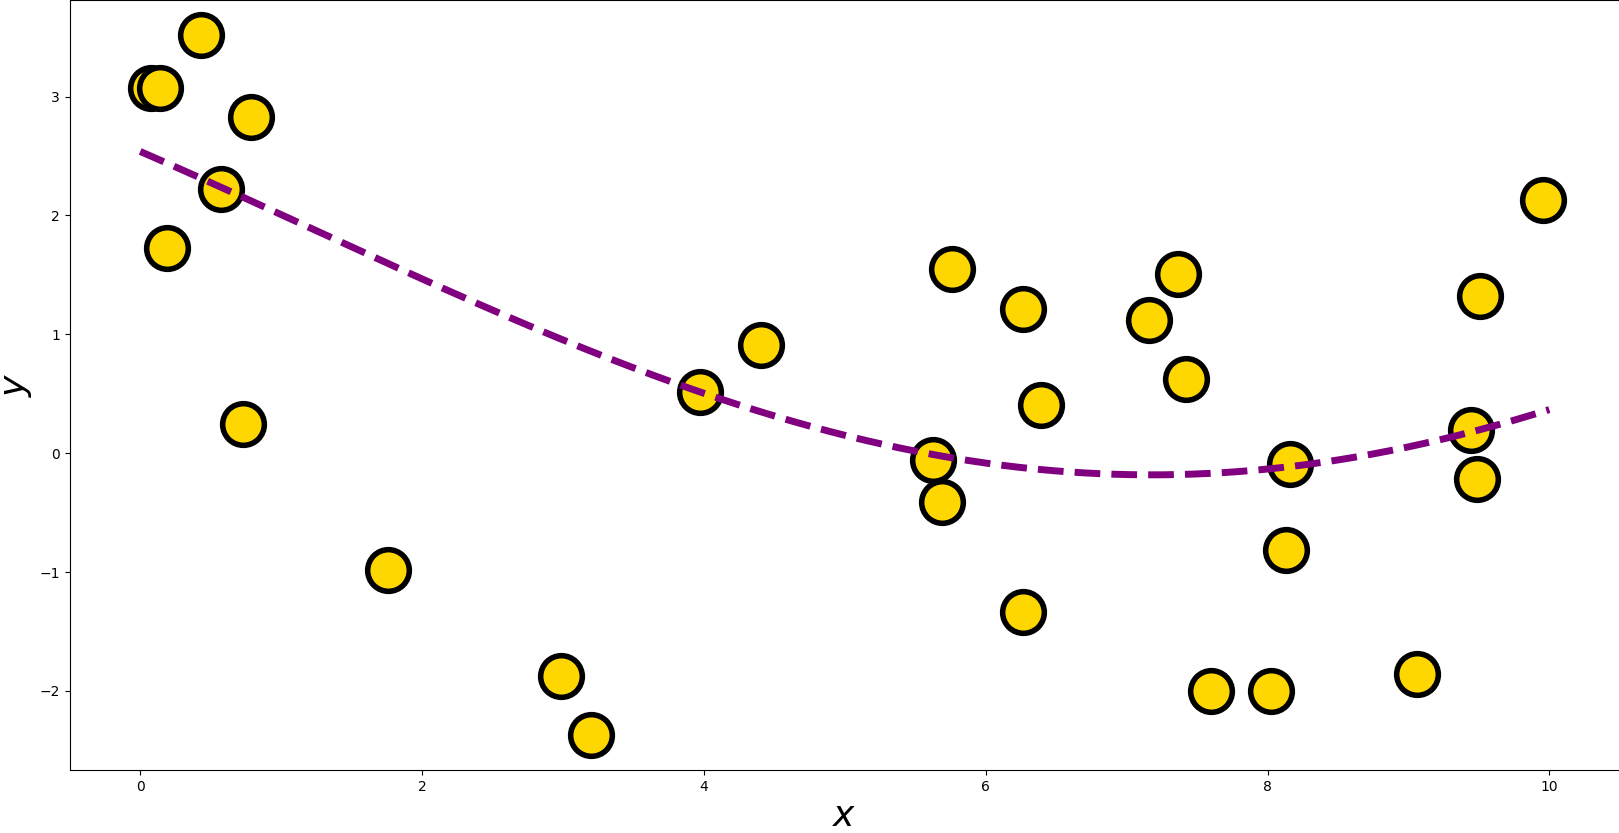
\includegraphics[width=\textwidth]{../figures/best_nonlinear.png}
\end{figure}

\column{0.5\textwidth}

\begin{alertblock}{Problem}

\begin{itemize}
\item Nonlinearity has introduced local minima in the loss surface
\item Gradient descent is getting stuck in those minima
\end{itemize}

\end{alertblock}

\end{columns}
 
 
% GOOD tutorial on optimizers
% https://mlfromscratch.com/optimizers-explained/#/


\end{frame}

\begin{frame}
\frametitle{Loss Surface}

We plotted the loss of the model as a function of $\beta_1$ and $\gamma_1$, holding the other two parameters at zero.

 \begin{figure}
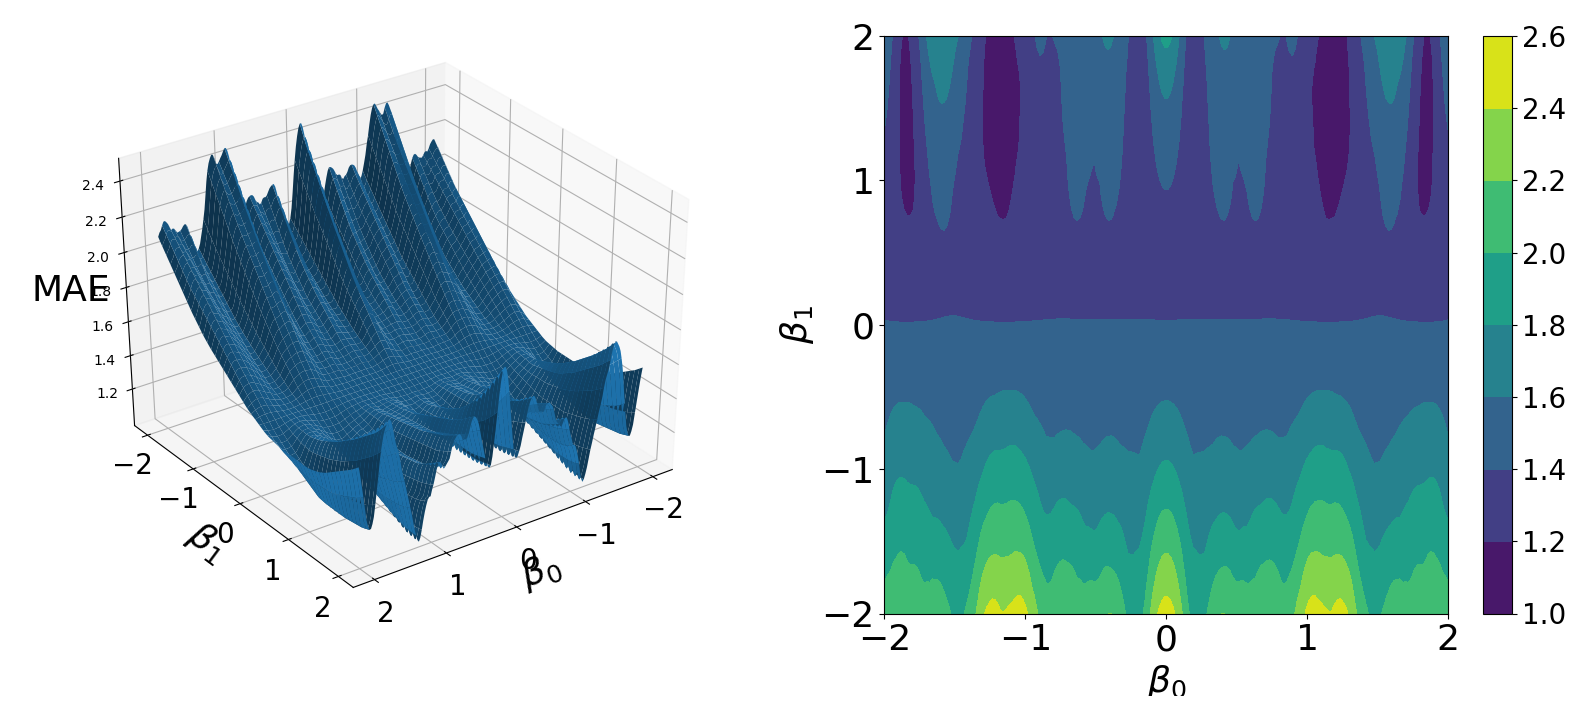
\includegraphics[width=0.8\textwidth]{../figures/nonlinear_loss.png}
\end{figure}

\begin{block}{Observation}

\begin{itemize}
\item Solution depends on initialization (where you start from)
\item May need to do multiple restarts
\end{itemize}

\end{block}

\end{frame}

\begin{frame}
\frametitle{Congratulations!}

\begin{itemize}
\item What you have just implemented is a very simple neural network with one \emph{hidden} neuron, the $cos()$ function, and one \emph{output} neuron.
\item The algorithm used to train a neural network is called ``Backpropagation'' and as you have just seen, it is simply gradient descent.
\end{itemize}

Backpropagation consists of a forward and backward pass:

\begin{itemize}
\item \textbf{Forward pass} is easy: just apply the mathematical function defined by the network on the inputs, while keeping track of all intermediate results. 
\item \textbf{Backward pass} requires the gradients. Here, the intermediate results kept from the forward pass are used to compute the values of the partial derivatives of the loss with respect to the parameters.
\end{itemize}






\end{frame}

\end{document}